\chapter{Diseño de la aplicación}

En este capítulo veremos cómo construir una aplicación para realizar el problema de clasificación utilizando redes parenclíticas.\\

En primer lugar veremos cuál es la arquitectura de la aplicación, posteriormente, qué tecnologías hemos utilizado para desarrollar esta aplicación y, por último describiremos las funcionalidades de la aplicación.

\section{Arquitectura de la aplicación}

La arquitectura de la aplicación está basada en una arquitectura clásica cliente-servidor, en la que en el lado del servidor se utiliza R como lenguaje de programación, como servidor web actúa RStudio Server, y Shiny como framework web para R. En el lado del cliente se usa ShinyDashboard.

\begin{figure}[htbp!]
	\centering
	\arquitectura
	\caption{Arquitectura de la aplicación}
	\label{fig:arquitectura}
\end{figure}

\section{Tecnología utilizada}

Como lenguaje de programación se ha utilizado R~\cite{R}, un lenguaje desarrollado para cálculos científicos y la realización de gráficas de alta calidad.

\begin{figure}[htbp!]
\centering

\includegraphics[width=0.3\linewidth]{imagenes/R}
\caption{Logo de R}
\label{fig:R}
\end{figure}

R incorpora la mayoría los test estadísticos más comunes, gran cantidad de funciones estadísticas y permite el manejo de datos de forma sencilla.\\

R es gratis y software open-source y tiene licencia GNU General Public License. R no tiene restricciones, por lo que puede ser usado cuando y donde se quiera e incluso es posible venderlo bajo las condiciones de la licencia.\\

R dispone de más de 8696 paquetes~\cite{Rpaquetes} disponibles de muchos repositorios especializados en diversas temáticas como minería de datos, econometría o bioestadística.\\

R es multipltaforma, por lo que está disponible en Windows, Mac y Linux, y dispone tanto de versiones de 32 como de 64 bits.\\

Como servidor web se ha utilizado RStudio Server~\cite{RStudioServer} que permite ver páginas web a través del lenguaje R. Dispone de dos licencias: Open Source Edition y Commercial. La primera permite acceso a través del navegador, y la segunda dispone de herramientas administrativas, autenticación y, métricas y sistemas de mantenimiento y gestión de recursos avanzados.\\

Como framework web se ha utilizado Shiny~\cite{Shiny}. Permite desarrollar aplicaciones web sobre R sin necesidad de conocer HTML, CSS o JavaScript. Shiny combina la interactividad (usando programación reactiva) con la potencia de cálculo de R.\\

\begin{figure}[htbp!]
	\centering
	
\includegraphics[width=0.3\linewidth]{imagenes/RShiny}
	\caption{Logo de Shiny}
	\label{fig:RShiny}
\end{figure}

Shiny Dashboard~\cite{ShinyDashboard} permite crear dashboards sobre aplicaciones Shiny de manera sencilla y rápida.\\

\begin{figure}
\centering
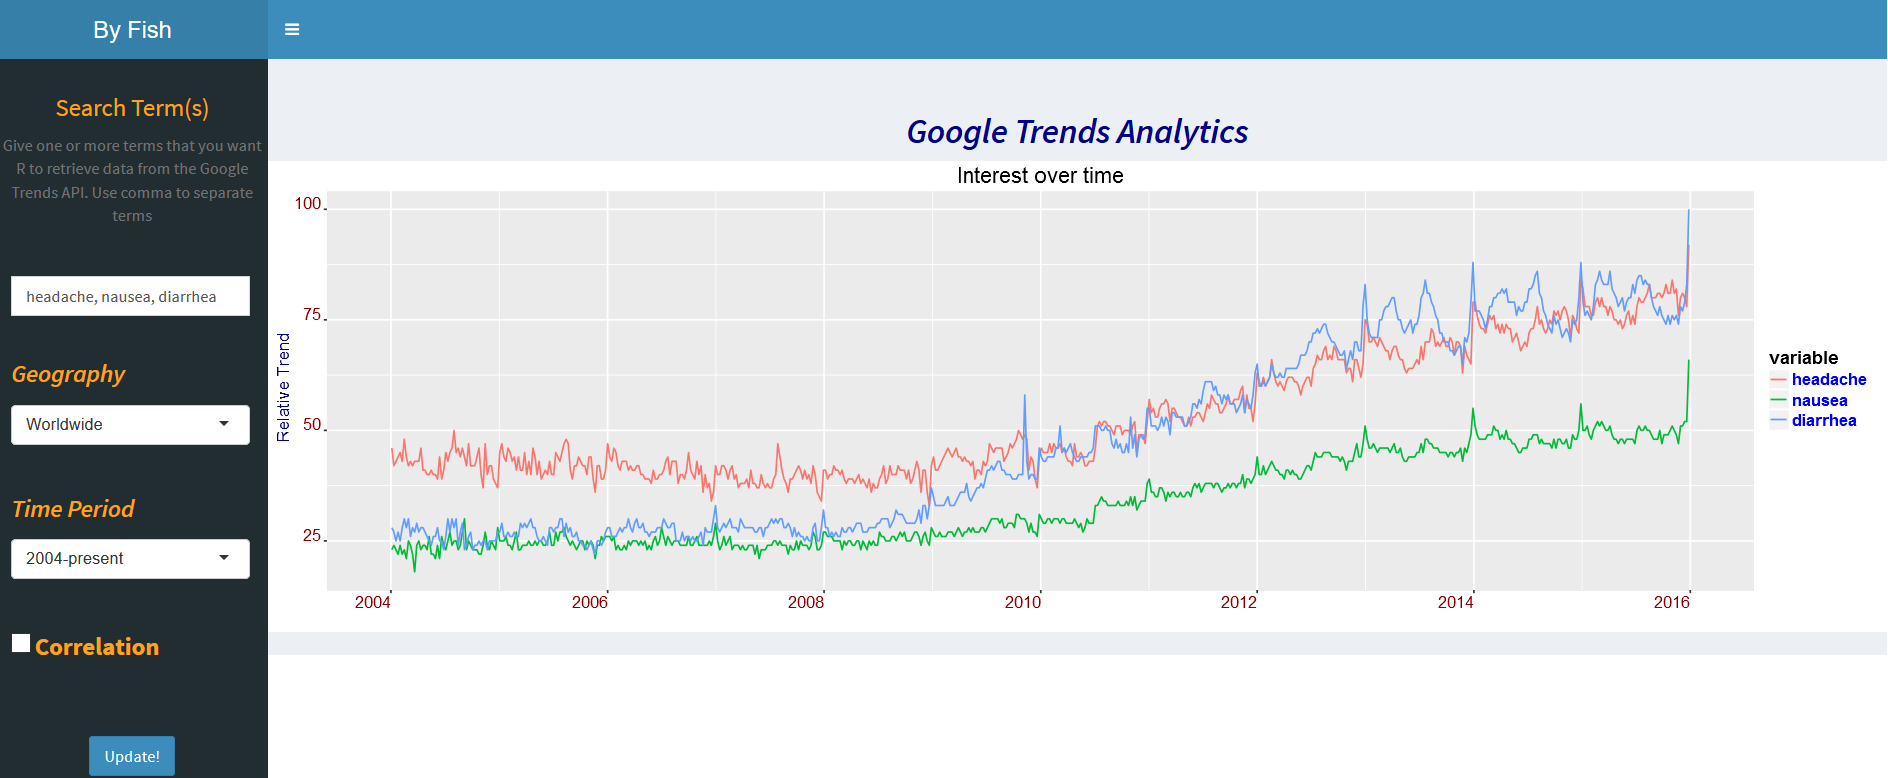
\includegraphics[width=0.7\linewidth]{imagenes/shinydashboard}
\caption{Dashborad realizado con Shiny Dashboard}
\label{fig:shinydashboard}
\end{figure}

Además, se han utilizado distintos paquetes de R:

\begin{enumerate}
	\item igraph~\cite{igraph}: análisis de grafos.
	\item e1071~\cite{e1071}: clasificación con Support Vector Machine.
	\item nnet~\cite{nnet}: clasificación con redes neuronales (con una sola capa oculta).
	\item rpart~\cite{rpart}: clasificación con árboles de decisión
	\item ggplot2~\cite{ggplot2}: librería para visualización. 
\end{enumerate}


La aplicación está dividida en una serie de scripts, entre los que se encuentran:

\begin{itemize}
	\item \textit{calculatePrediction}: realiza las predicciones a partir del cálculo de las redes parenclíticas, calculando las medidas dadas por las Ecuaciones~\ref{eq:densidad}~,~\ref{eq:clustering}~,~\ref{eq:eficiencia}~y~\ref{eq:camino} y aplica una red neuronal para realizar la clasificación.
	
	\item \textit{calculateML}: aplica redes neuronales, Support Vector Machine y árboles de decisión para realizar la clasificación de unos datos dados.
	
	\item \textit{drawParencliticNetwork}: representa una red parenclítica con el uso del paquete \textit{igraph}.
	
	\item \textit{drawRegressionLine}: representa las curvas de regresión (lineal, exponencial, cuadrática y recíproca) de un par de variables del conjunto de entrada.
	
	\item \textit{drawNormalPlot}: representa las distribuciones normales de cada clase. 
\end{itemize}

Las características principales de la aplicación son:

\begin{itemize}
	\item Clasificación usando redes parenclíticas aplicando modelos lineal, exponencial, cuadrático y recíproco.
	
	\item Clasificación usando métodos clásicos de machine learning como redes neuronales, Support Vector Machine y árboles de decisión.
	
	\item Visualización de estadísticas descriptivas de las variables cuantitativas, tanto de forma global como por grupo.
	
	\item Generación de informes.
\end{itemize}


\section{Un paseo por la aplicación}

La página de inicio se muestra en la Figura~\ref{fig:inicio}. En la parte izquierda se muestran todas las pestañas disponibles de la aplicación, y en la parte derecha se muestra el contenido de cada pestaña. En este caso, se muestra un formulario para subir el fichero de datos. Este fichero deberá estar en formato CSV y los datos deberán estar separados por coma.\\

\begin{figure}[tbph!]
	\centering
	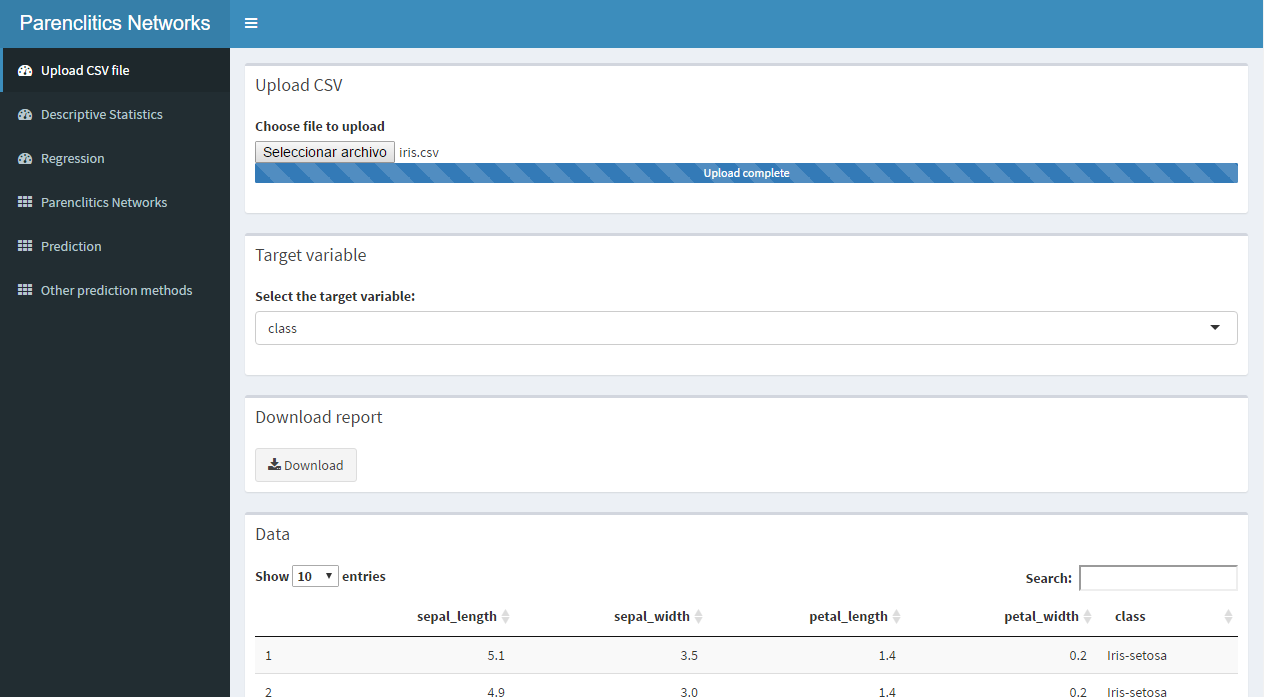
\includegraphics[width=0.7\linewidth]{imagenes/inicio}
	\caption{Página de inicio de la aplicación}
	\label{fig:inicio}
\end{figure}

Una vez cargados los datos, se muestran las variables que pueden ser usadas para la clasificación, es decir, aquellas que sean del tipo factor.\\

En la parte inferior de la pantalla se muestran los datos cargados en forma de tabla. Es posible ordenar las columnas por orden creciente o decreciente y buscar algún datos en el conjunto de datos.\\

En la pestaña Regression (Figura~\ref{fig:regresion}) se representan para cada par de variables sus curvas de regresión (lineal, exponencial, cuadrática y recíproco). 

\begin{figure}[tbph!]
	\centering
	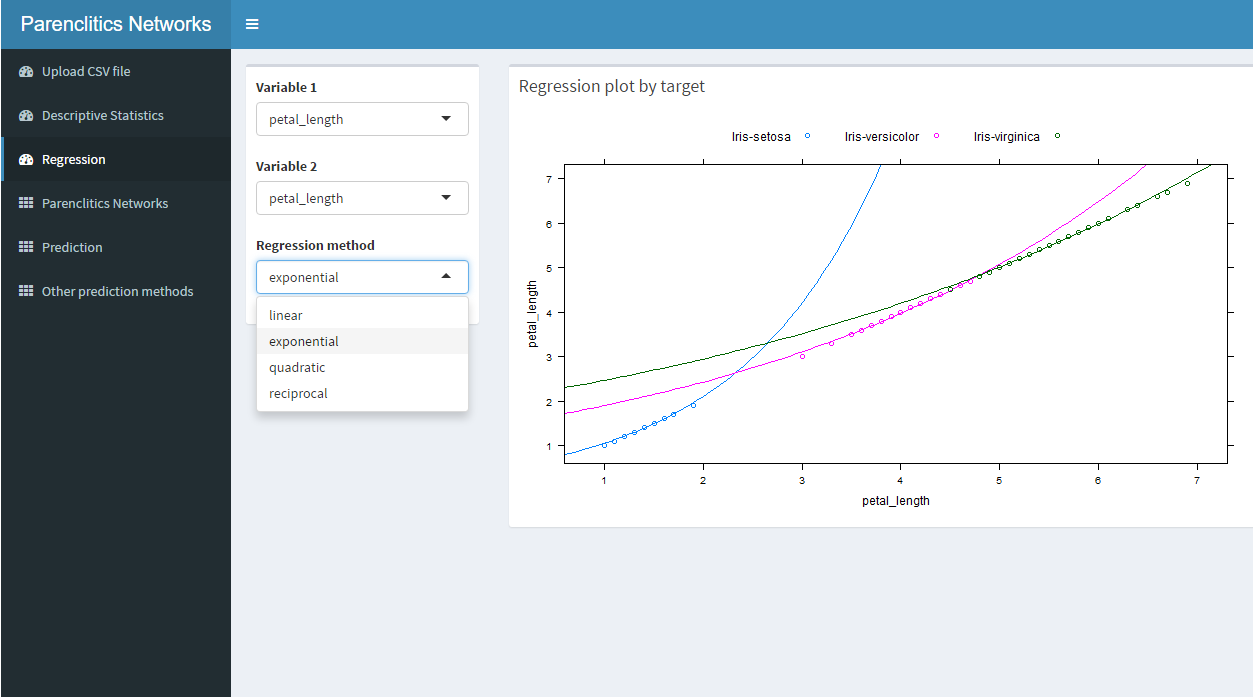
\includegraphics[width=0.7\linewidth]{imagenes/regresion}
	\caption{Pestaña Regression}
	\label{fig:regresion}
\end{figure}

En la pestaña Parenclitic Network (Figura~\ref{fig:pn}), se pueden ver las distribuciones de cada clase, calculadas a partir del modelo de regresión deseado y la red parenclítica de cada observación (Figura~\ref{fig:parencliticNetwork}). 

\begin{figure}[tbph!]
	\centering
	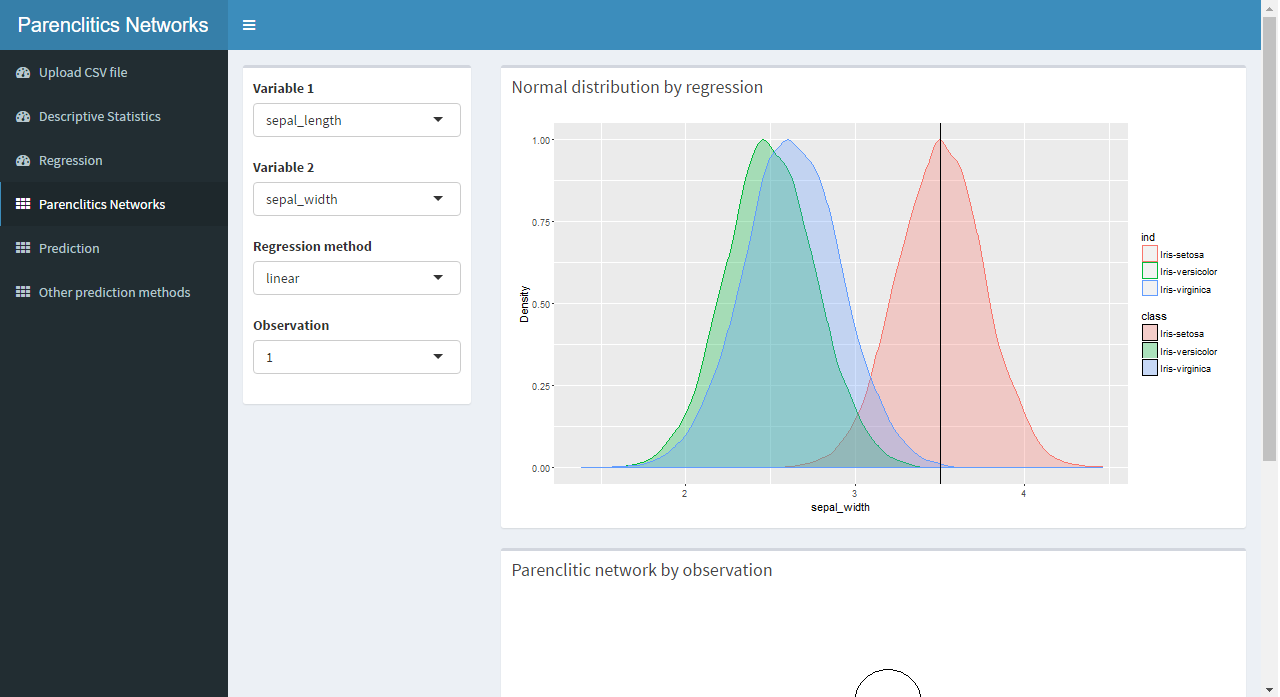
\includegraphics[width=0.7\linewidth]{imagenes/pn}
	\caption{Pestaña Parenclitic Network}
	\label{fig:pn}
\end{figure}

\begin{figure}[tbph!]
	\centering
	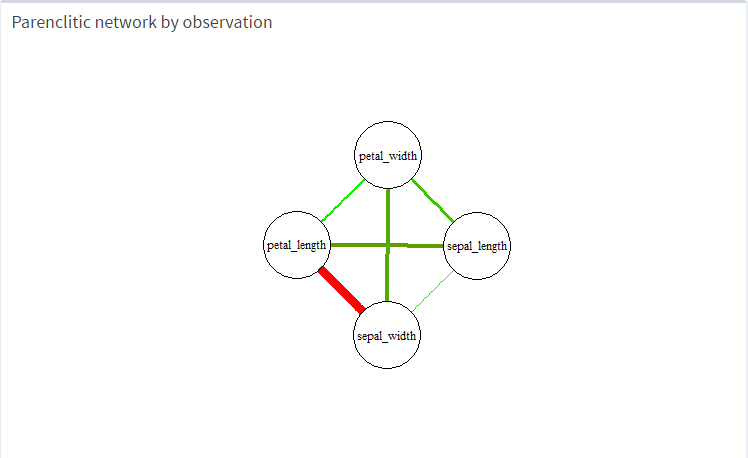
\includegraphics[width=0.7\linewidth]{imagenes/parencliticNetwork}
	\caption{Red parenclítica}
	\label{fig:parencliticNetwork}
\end{figure}

En la pestaña Prediction se muestran las gráficas de las medidas obtenidas de las redes parenclíticas (Figura~\ref{fig:medidas}) así como la clasificación realizada a partir de estas medidas (Figura~\ref{fig:clasificacion}).\\

\begin{figure}[tbph!]
	\centering
	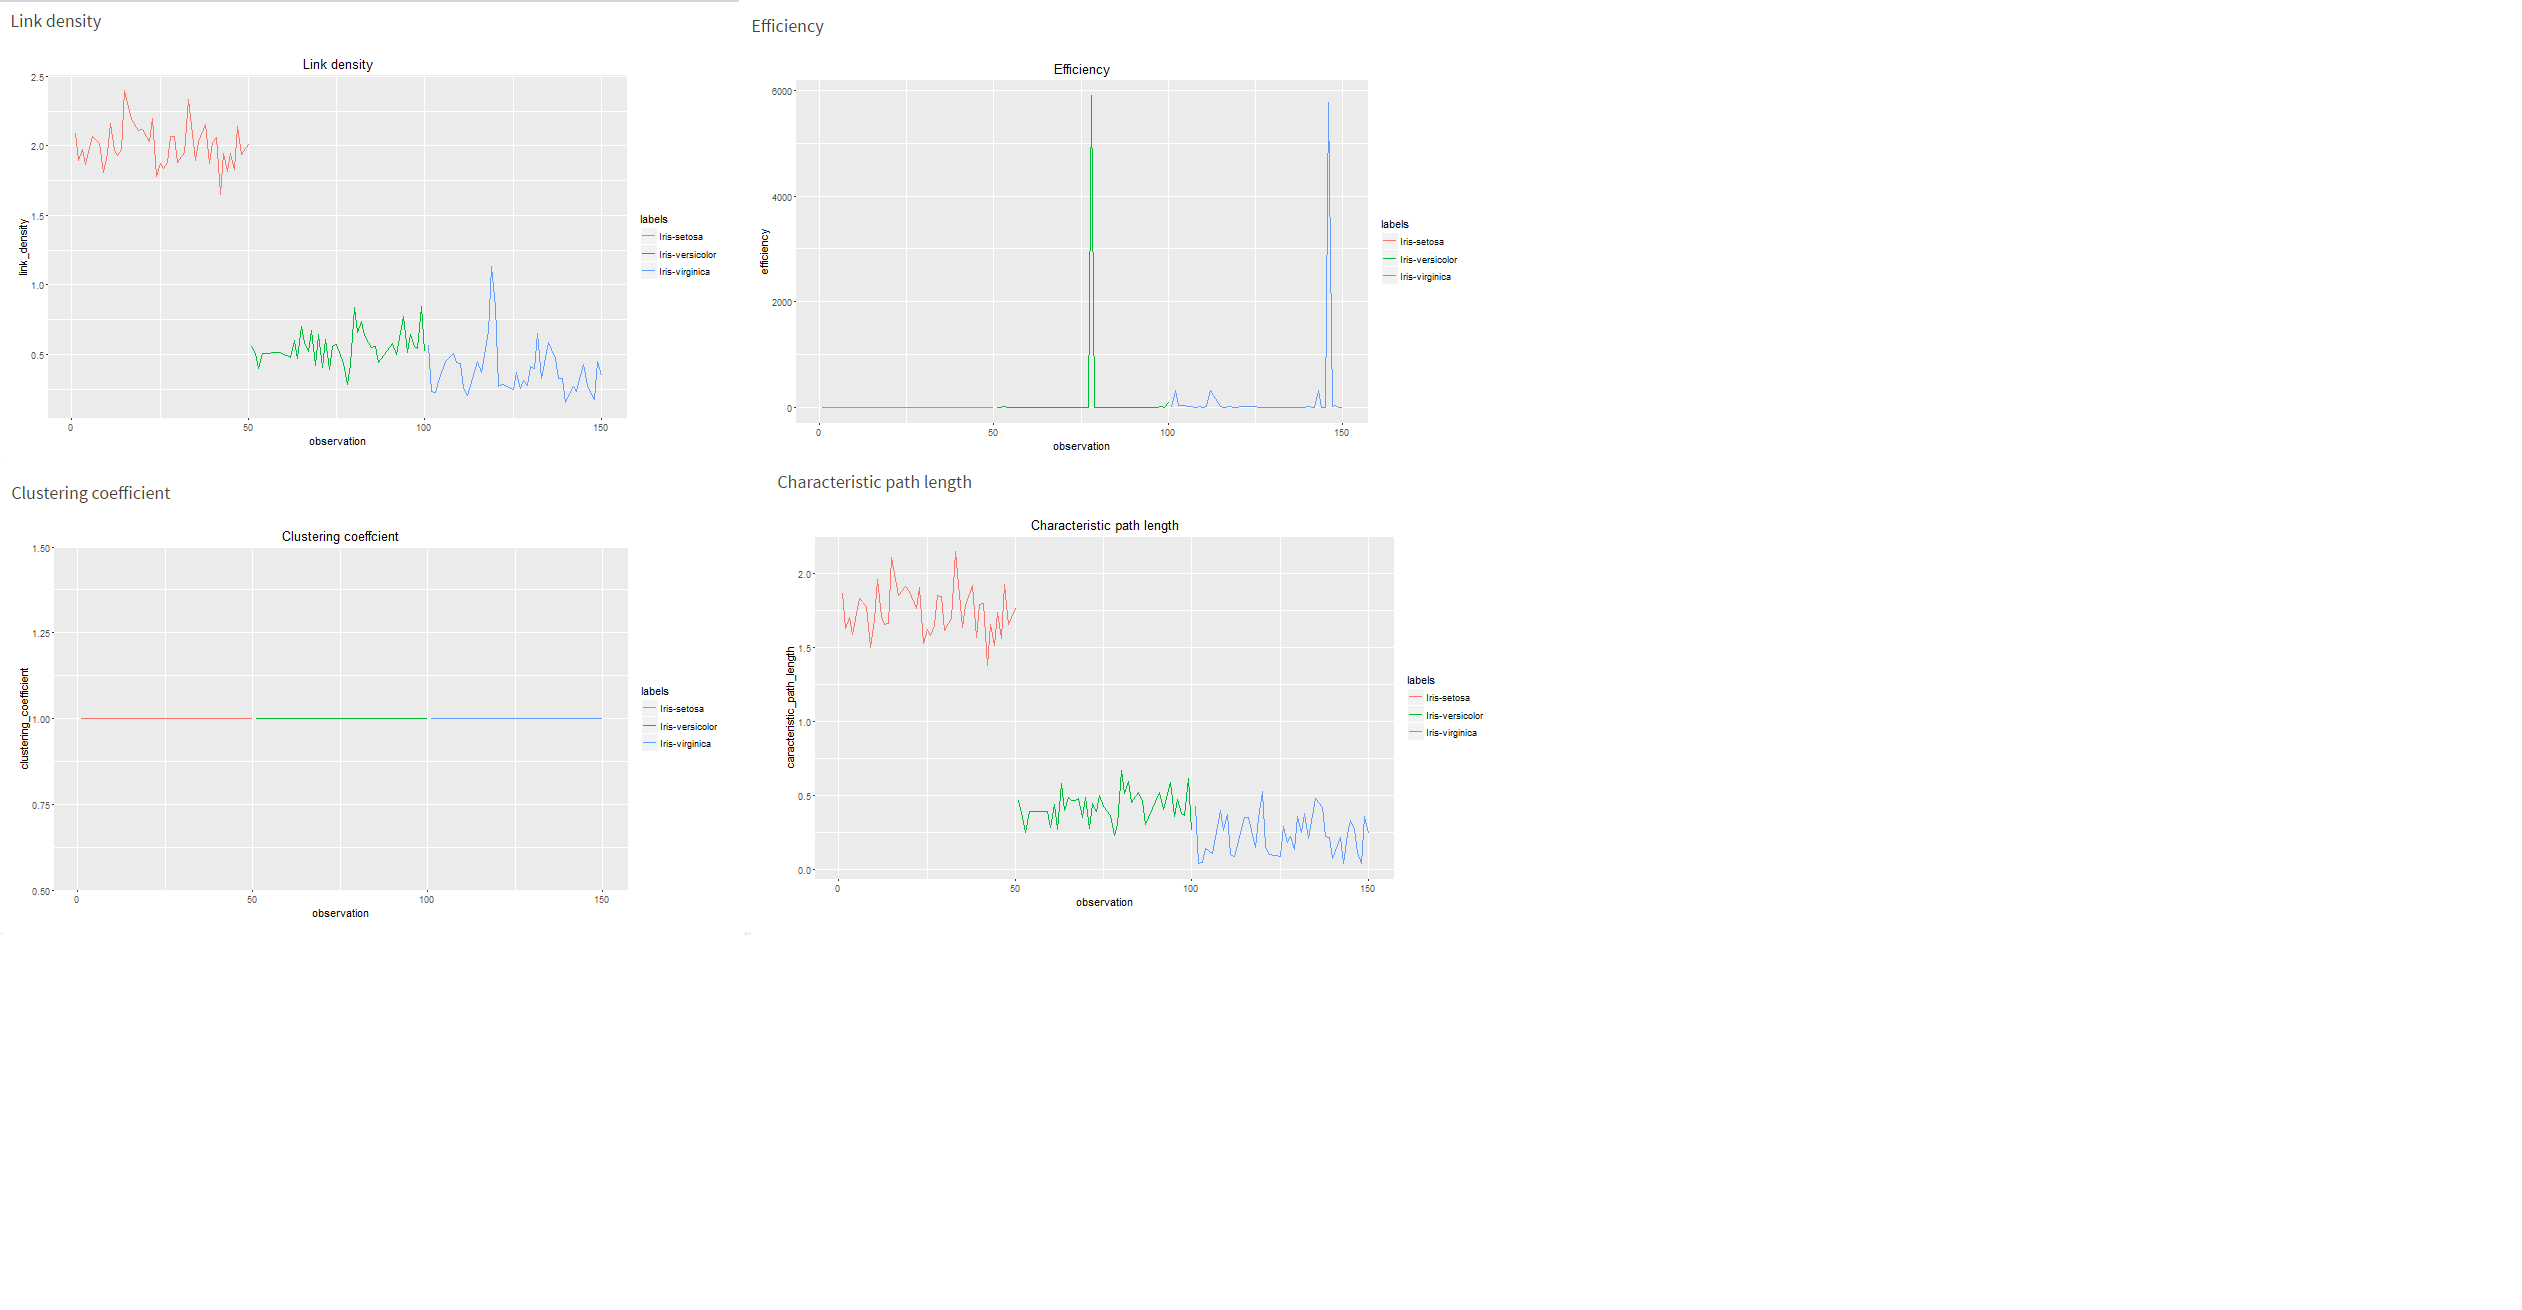
\includegraphics[width=0.7\linewidth]{imagenes/medidas}
	\caption{Medidas}
	\label{fig:medidas}
\end{figure}

\begin{figure}[tbph!]
	\centering
	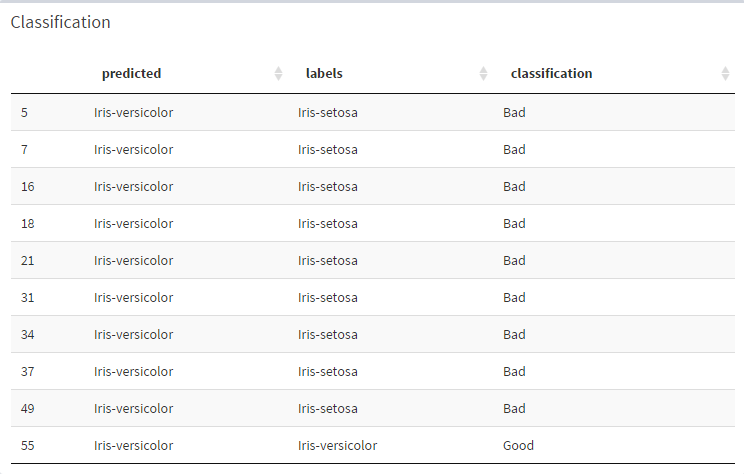
\includegraphics[width=0.7\linewidth]{imagenes/clasificacion}
	\caption{Clasificación con redes parenclíticas}
	\label{fig:clasificacion}
\end{figure}

Por último en la pestaña Other prediction methods, se obtiene la clasificación mediante redes neuronales, Support Vector Machine y árboles de decisión (Figura~\ref{fig:prediccionML}) de los datos iniciales.\\

\begin{figure}[tbph!]
	\centering
	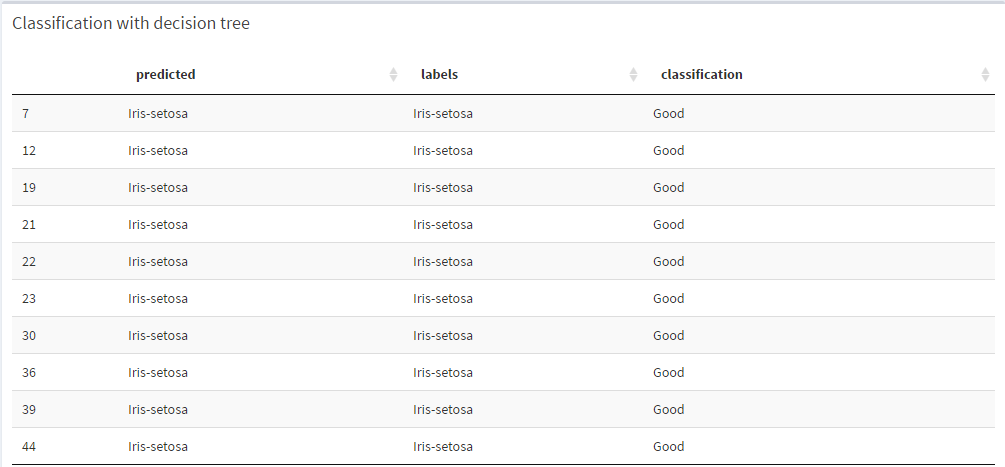
\includegraphics[width=0.7\linewidth]{imagenes/prediccionML}
	\caption{Predicción usando árboles de decisión}
	\label{fig:prediccionML}
\end{figure}

En el próximo capítulo aplicaremos esta aplicación a una serie de conjuntos de datos.